\documentclass[a4paper]{scrartcl}

\parindent0cm

\usepackage[T1]{fontenc} 
\usepackage[utf8]{inputenc}
\usepackage[ngerman]{babel}
\usepackage{pdflscape}
\usepackage{pdfpages}
\usepackage{latexsym}
\usepackage{color}
\usepackage{booktabs,makecell,tabularx}
\usepackage{amsmath}
\usepackage{amssymb}
\usepackage{graphicx}
\usepackage[colorlinks,linkcolor = blue]{hyperref}
\usepackage{siunitx}  
\sisetup{locale = DE}
\usepackage{enumitem}

\usepackage[left=2.5cm,right=2.5cm,top=2.5cm,bottom=2cm]{geometry}

%Hintergrundbild der Titelseite
\usepackage{eso-pic}
\newcommand\BackgroundPic{%
\put(0,0){%
\parbox[b][\paperheight]{\paperwidth}{%
\vfill
\centering

\includegraphics[width=\paperwidth,height=\paperheight,%
keepaspectratio]{background.png}%
\vfill
}}}

%\usepackage{showframe}

\begin{document}

% Titelseite    
\newpage
\thispagestyle{empty}
\AddToShipoutPicture*{\BackgroundPic}

\newgeometry{top=0.6cm, bottom=2.04cm, left=2.24cm, right=2.24cm}

\begin{center}

\begin{tabular}{p{3cm}p{8cm}p{4cm}}
&\textcolor{red}{\LARGE{ }} & \vspace{-0.5cm} 
\includegraphics[height=1.4cm]{Logo_Titelseite_ohne_text.png}\\
\end{tabular}

\begin{tabular}{p{5cm}p{10.5cm}}
&\\
&
\includegraphics[height=0.9cm]{Logo_Titelseite_ohne_Symbol.png}\\
\end{tabular}

\end{center}

\vspace{7cm}

\begin{flushright}
\begin{Huge}
\textbf{Dokumentation Bachelorprojekt} \\
\end{Huge}
\vspace{2cm}
\Large{Heiko Nöldeke, Marc Bolsch, Pascal Roschkowski, Philipp Otto} \\
\vspace{0.5cm}
\LARGE{\textbf{Entwurf und Ausarbeitung eines \\ Traffic-Noise-Detector-Prototypen}}
\end{flushright}
\vspace{8cm}

\begin{center}
\begin{tabular}{lp{2cm}r}
Fakultät Technik und Informatik && Faculty of Engineering and Computer Science \\
Departement Mechatronik && Departement of Mechatronic Engineering \\
\end{tabular}
\end{center}

\newpage
\restoregeometry

\ClearShipoutPicture
\thispagestyle{empty}
\newgeometry{top=6cm, bottom=2.04cm, left=2.24cm, right=2.24cm}

\begin{center}
\Large{\textbf{Heiko Nöldeke, Marc Bolsch, Pascal Roschkowski, Philipp Otto}} \\  
\vspace{1.5cm}
\LARGE{\textbf{Traffic-Noise-Detector-Prototyp}}
\end{center}

\vspace{14cm}

\begin{tabular}{l}
Bachelorprojekt eingereicht im Rahmen der Bachelorprüfung \\
\\
im Studiengang Mechatronik \\
am Departement Fahrzeugtechnik und Flugzeugbau \\
der Fakultät Technik und Informatik \\
der Hochschule für Angewandte Wissenschaften Hamburg\\
\\
Erstprüfer: Prof. Dr. Rasmus Rettig\\
\\
Abgabedatum: \today
\end{tabular}

\newpage
\restoregeometry
\tableofcontents
\thispagestyle{empty}
\newpage

\setcounter{page}{1}

\section{Vorwort}

Im Rahmen eines Bachelors Projekts im Fachbereich Mechatronik an der HAW Hamburg, ist eine kleine Gruppe Studierender dazu beauftragt, eine praxisnahe Aufgabe zu lösen. Dazu gehört der Prozess der Produktentwicklung, aber auch die Erschaffung eines Prototypen. Diese Dokumentation dient dazu, die Arbeitsschritte und eine Produktbeschreibung festzuhalten. Auf der Basis der Arbeit von Maximilian Welz führen die vier genannten Autoren unter Leitung von Herrn Prof. Dr. Rasmus Rettig eine Anpassung des <Bezeichnung> an die neue Aufgabenstellung an.
\newpage

\section{Git}
\begin{tabular}{|l|l|}
\hline
Git-Befehl & Auswirkung\\
\hline
\hline
git clone plus Link & Git-Verzeichnis auf PC klonen\\
\hline
git pull & aktuellen Stand vom Server holen\\
\hline
git status & Informationen über den aktuellen Stand\\
\hline
git add & geänderte Dateien hinzufügen mit Dateiname\\
\hline
git add . & alle geänderten Dateien hinzufügen\\ 
\hline
git commit -m \glqq Kommentar\grqq & Commit erstellen\\
\hline
git push & auf den Sever schieben\\
\hline
\end{tabular}

\newpage

\section{Zusammenfassung der Aufgabenstellung}

\begin{tabular}{|p{15cm}|}
\hline
\textbf{Project Charter:} Traffic-Noise-Detector (Lärmblitzer), Bachelor Project - Hr. Otto, Hr. Nöldeke, Hr. Bolsch, Hr. Roschkowski\\
\hline
\textbf{Mission:} Aufbau eines Prototypen zur Erkennung und Lokalisierung von Fahrzeigen mit (zu) hoher Lärm Emission (z. B. \url{https://www.auto-motor-und-sport.de/verkehr/laerm-blitzer-in-europa-fallen-gegen-auto-poser/}).\\
\hline
\textbf{Deliverables (incl. timing):}
\begin{itemize}
\item Anforderungsentwicklung (Mechanisch, Akustisch, Elektrisch, Algorithmisch)
\item Systematische Auswahl / ggf. Kombination oder Weiterentwicklung
\item Realisierung
\item Test und Bewertung der Eignung
\item Überarbeitung basierend auf den Testergebnissen [T0+6 Wochen]
\item Abschlussintegration, Demonstration/Vortag und Dokumentation [T0+12 Wochen]
\end{itemize}\\
\hline
\textbf{Expected Scope / Approach / Activities:}
\begin{itemize}
\item Einarbeitung in das Messsystem und die Programmierumgebung
\item Einarbeitung in den Stand der Technik von Algorithmen zur Erkennung und Lokalisierung akustischer Signale
\item Zielgerichtete Auswahl, Weiterentwicklung / Kombination im Hinblick auf genutzte Hardware sowie die Erkennung mit einer hohen Erkennungsrate
\end{itemize}\\
\hline
\textbf{Strategic alignment factors:}
\newline
Integration in dei Arbeitsgruppe Urban Mobility Lab mit den laufenden Arbeiten\\
\hline
\textbf{Timeframe/Duration:}
\begin{itemize}
\item Start 1.10.2020 (Vorbereitung
\item Abschluss 30.3.2021 (gerne früher)
\end{itemize}\\
\hline
\textbf{Team Resources:}
\newline
Nutzung Labor Stiftstraße 69 Raum 109 mit der dort verfügbaren Infrastruktur (Elektronikentwicklung, Software Entwicklung, Server, Löteinrichtung; Kamera, Testfahrzeug, Rechner)\\
\hline
\textbf{Team Process:}
\begin{itemize}
\item Reglmäßige Reviews (14 tägig)
\item Optional: Teilnahme am Teammeeting
\end{itemize}\\
\hline
\end{tabular}

\newpage

\section{Brainstorming}

Im Rahmen des Projekts wird anhand des stationären Blitzers am Anckelmannsplatz (Hamburg, Deutschland) eine mögliche Arbeitsumgebung erarbeitet.

\begin{figure}[h]
\centering

\includegraphics[scale=0.2]{Sections/Brainstorming/Blitzer.jpeg}
\caption{Blitzer Anckelmannsplatz}
\label{fig:Blitzer_Anckelmannsplatz}
\end{figure}

\begin{figure}[h]
\centering

\includegraphics[scale=0.2]{Sections/Brainstorming/Blickwinkel_Blitzer_2.jpeg}
\caption{Blitzer Blickwinkel}
\label{fig:Blitzer_Blickwinkel}
\end{figure}

\newpage

\begin{figure}[h]
\centering
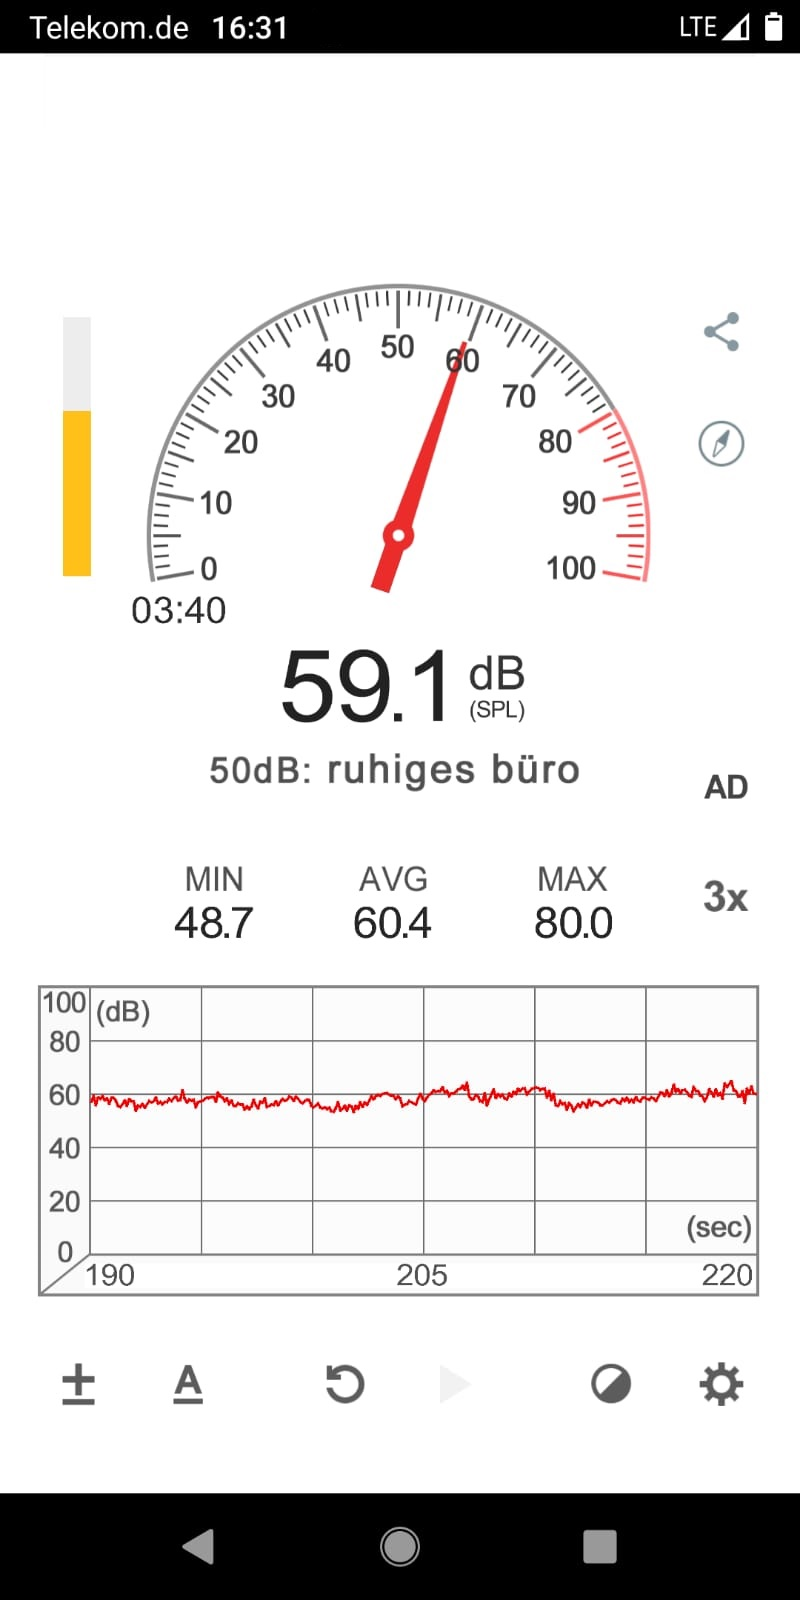
\includegraphics[scale=0.15]{Sections/Brainstorming/Pegelmessung_Anckelmannsplatz_am_Blitzer_Nachmittag.jpeg}
\caption{Schallmessung}
\label{fig:Schallmessung}
\end{figure}

Bild \ref{fig:Blitzer_Anckelmannsplatz} und \ref{fig:Blitzer_Blickwinkel} zeigen den oben genannten Blitzer, sowie den anzunehmenden Blinkwinkel. Öffnungswinkel des Detectors müssen noch erörtert werden. \\
\noindent Bild \ref{fig:Schallmessung} zeigt eine Schallmessung an einem gewöhnlichen Donnerstagnachmittag auf dem Anckelmannsplatz Höhe des Blitzers als Referenz des Pegelwertes.

\newpage

%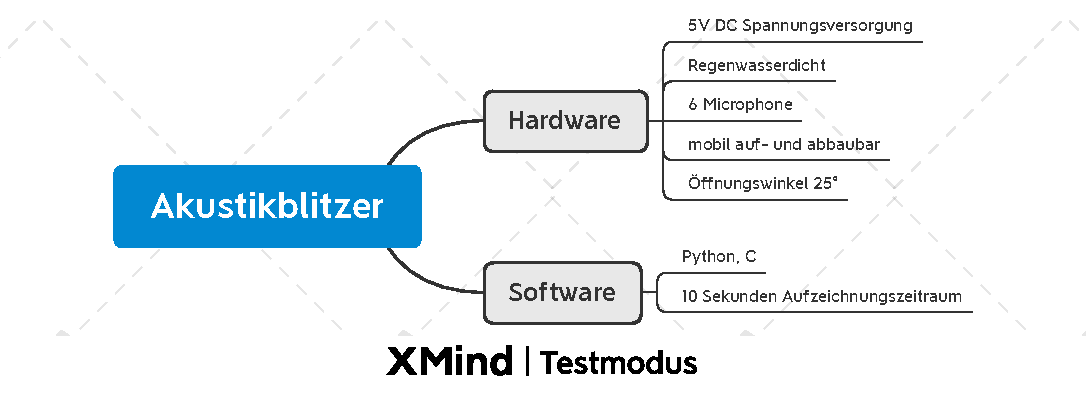
\includepdf[pages=-]{Sections/Brainstorming/2020-10-15_Brainstorming}

\newpage

\section{Meeting 22. 10. 2020}

Ort: Zoom-Online-Meeting
\newline
Zeit: 13:00 Uhr
\newline
Meeting-ID: 951 5710 6731
\newline
Kenncode: 179320
\newline
Protokollant: 
\newline
Vorläufige Themenauswahl:
\begin{itemize}
\item Ihre (unsere) Fragen
\item Zeitplanung
\item HW, SW
\item Verteilung der Aufgaben
\item weiteres:
\end{itemize}

\vspace{2cm}
\noindent
unsere Fragen:
\begin{enumerate}
\item Soll die Datenauswertung zeitgleich mit der Aufnahme erfolgen? \hfill $\Box$ Ja\qquad $\Box$ Nein
\item Wird die Berechnung intern auf dem Paspberry Pi ausgeführt? \hfill $\Box$ Ja\qquad $\Box$ Nein
\item Bekommen wir die Dokumentation und den Source Code des Schussdetektors heute noch? \hfill $\Box$ Ja\qquad $\Box$ Nein
\item Welche Art von Kamera soll in diesem System verwendet werden?
\item Welche Brennweite/ Öffnungswinkel ist gefordert?
\item Wie wird die Dämpfung trotz hoher IP Schutzklasse umgangen?
\item Mit welcher maximalen Fahrgeschwindigkeit muss das System zurechtkommen?
\item Ist ein 24h Betrieb gefordert? \hfill $\Box$ Ja\qquad $\Box$ Nein
\item Ab welchem Lautstärkepegel soll das System anschlagen?
\item Wie viele Fahrzeuge sollen simultan erfasst werden?
\item Wie viele Fahrspuren soll ein System überwachen?
\item Welche Wetter- und Temperaturverhältnisse soll das System vertragen können?
\item Soll das System erweiterbar sein? \hfill $\Box$ Ja\qquad $\Box$ Nein
\item Soll das System Redundanzen besitzen? \hfill $\Box$ Ja\qquad $\Box$ Nein
\item Soll das System mobil ausgelegt werden? \hfill $\Box$ Ja\qquad $\Box$ Nein
\item Nach welchen Umwelt und Recycling Standards arbeiten wir?
\item In welchem Bereich liegen die Messtoleranzen?
\item Welche Fehlerwahrscheinlichkeit ist akzeptabel?
\item Soll eine Fernwartung / ein Fernzugriff möglich sein? \hfill $\Box$ Ja\qquad $\Box$ Nein
\item Mit welcher Messfrequenz wird das System arbeiten?
\item Muss bei der Entwicklung auf Servicemaßnahmen geachtet werden? \hfill $\Box$ Ja\qquad $\Box$ Nein
\item Welche Rahmenbedingungen gelten für die Dokumentation?
\item Welche Möglichkeiten haben wir in der Werkstatt?
\end{enumerate}
\newpage

\section{Anforderungsanalyse}

\subsection{Lastenheft}

Es soll ein Prototyp für die Erkennung und Lokalisierung eines Kraftfahrzeuges mit (zu) hohen Lärmemissionen entwickelt werden. Dabei sollen innerorts bis \SI{50}{km/h} mindestens drei Fahrspuren, mit einer Option auf zwei weitere, abgedeckt werden. Der Detektor soll so konstruiert werden, dass er problemlos von einer einzelnen Person in einem handelsüblichen Rucksack verstaut und transportiert werden kann. Die mindestens verfügbare Einsatzdauer soll eine halbe Stunde betragen. Die im Einsatz erfassten Daten sollen innerhalb von zwei Sekunden an Peripheriegeräte gesendet werden, um dort von dem Benutzer kontrolliert werden zu können. Der Benutzer kann sich in einem Aktionsradius von maximal \SI{30}{m} befinden und soll die Möglichkeit der Fernwartung haben. Die Messtoleranz des Prototypen soll im Bereich von \SI{0,5}{m} und \SI{1}{m} liegen. Eine Fehlerwahrscheinlichkeit von 99\% soll erreicht werden. (\color{red}Den letzten Punkt bitte nochmal überdenken - Sinnprüfung\color{black}) Die Messung soll mit einer Messfrequenz von \SI{48}{kHz} bei 24 Bit durchgeführt werden.

\section{Pflichtenheft}

Bei der Erstellung des Pflichtenhefts wurde, basierend auf dem Lastenheft des Traffic-Noise--Detectors, auf die individuellen Forderungen des Auftraggebers eingegangen. Die daraus entstandenen Umsetzungen sind aus der folgenden Tabelle zu entnehmen:

\begin{center}
\begin{tabular}{|p{2cm}|p{6cm}|p{6cm}|}
\hline
\textbf{Ifd.-Nr} & \textbf{Anforderungen gemäß Lastenheft:} & \textbf{Umsetzung im Pflichtenheft:}\\
\hline
1 & Überwachung von drei Fahrspuren & Mit Hilfe von sechs Mikrophonen, welche durch den Auftraggeber bereitgestellt werden.\\
\hline
2 & Angemessenes Gewicht & Benötigte Halterungen/ Vorrichtungen werden bevorzugt mittels eines 3D-Druckverfahrens hergestellt, um so das Gewicht zu senken. \hfill\\
\hline
3 & Verstaubar in einem Rucksack & Ein entsprechendes Gehäuse wird durch den Auftraggeber zur Verfügung gestellt. \\
\hline
4 & Leicht aufbaubar & Als Unterbau wird ein Stativ aus dem Fotografie Bereich verwendet. Dieses verfügt bereits über eine passende Aufnahme für den Prototypen.\\
\hline
5 & Einsatzdauer > 0.5 Stunden & Die Energieversorgung wird mittels Akkumulatoren sichergestellt \\
\hline
6 & Übertragung der erfassten Daten in einem Aktionsradius von \SI{30}{m} & WLAN Netz \\
\hline
7 & Betreiben einer Fernwartung & WLAN Netz\\
\hline
8 & Messtoleranz im Bereich \SI{0,5}{m} und \SI{1}{m} & \\
\hline
9 & Fehlerwahrscheinlichkeit von 99\% & \\
\hline
10 & Die Messfrequenz soll \SI{48}{kHz} bei 24 Bit betragen \hfill & Das System wird entsprechend eingestellt \hfill \\
\hline
11 &&\\
\hline
12 &&\\
\hline
13 &&\\
\hline
14 &&\\
\hline
&&\\
\hline
&&\\
\hline
\end{tabular}
\end{center}
\end{document}